\documentclass[conference]{IEEEtran}
\usepackage{amsmath,amssymb,amsfonts}
\usepackage{algorithmic}
\usepackage{graphicx}
\usepackage{textcomp}
\usepackage{xcolor}
\usepackage[style=ieee]{biblatex}
\addbibresource{refs.bib}

\begin{document}
\title{Characterizing hippocampal replay using hybrid point process state space models}

\author{\IEEEauthorblockN{1\textsuperscript{st} Eric L. Denovellis}
\IEEEauthorblockA{\textit{Howard Hughes Medical Institute and}\\
\textit{Dept. of Physiology}\\
\textit{Univ. of California, San Francisco}\\
San Francisco, CA, USA \\
https://orcid.org/0000-0003-4606-087X}
\and
\IEEEauthorblockN{2\textsuperscript{nd} Loren M. Frank}
\IEEEauthorblockA{\textit{Howard Hughes Medical Institute}\\
\textit{Kavli Institute for Fundamental Neuroscience and}\\
\textit{Dept. of Physiology} \\
\textit{Univ. of California, San Francisco}\\
San Francisco, CA, USA \\
loren@phy.ucsf.edu}
\and
\IEEEauthorblockN{3\textsuperscript{rd} Uri T. Eden}
\IEEEauthorblockA{\textit{Dept. of Mathematics and Statistics} \\
\textit{Boston University}\\
Boston, MA, USA \\
tzvi@bu.edu}

}

\maketitle

\begin{abstract}
In the hippocampus, replay sequences are temporally compressed patterns of neural spiking that resemble patterns that occur when the animal is moving through the environment. Because replay sequences typically occur when the animal is at rest, replay is hypothesized to be part of an internal cognitive process that enables the retrieval of past spatial memories and the planning of future movement. Traditionally, replay sequences have been discovered by identifying sharp wave ripples (SWRs)---high frequency oscillations that occur in association with replay---and then looking within SWRs for spatially continuous patterns of neural spiking. This does not fully account for the content or timing of replay sequences, however. Replay sequences do not always co-occur with sharp wave ripples, have more complex dynamics than spatially continuous movement, have different temporal ordering than during movement, and change based on task. In this work, we introduce a hybrid state space framework to describe the richness of replay sequences. We show how defining discrete latent states associated with continuous latent dynamics and point process observations allows us to identify when non-local replay sequences occur, categorize the type of sequence based on their inferred continuous dynamics, and decode the spatial trajectory corresponding to the replay sequence.

\end{abstract}

\begin{IEEEkeywords}
State-space methods, Hippocampus, Replay, Switching liner dynamical systems, Point process
\end{IEEEkeywords}

\section{Introduction}
A central question in neuroscience is how patterns of neuronal activity in the brain contribute to the formation and use of memories. This is a particularly difficult question because memory processes can engage an unobserved, internal state of mind which does not necessarily correspond to the animal's current behavior. Moreover, the associated neuronal activity patterns are noisy, high-dimensional, and can rapidly change on short timescales. As a result, neuroscientists need statistical methods that are flexible enough to capture the dynamically changing state of the brain, but remain interpretable enough to understand what those states are.

Take, for example, the phenomenon of hippocampal replay. In the hippocampus---a brain area known for its role in memory and early learning---neurons selectively respond based on position in the environment \cite{OKeefehippocampusspatialmap1971}, the population pattern of spiking activity reflecting the trajectory of the animal. When the animal is asleep or immobile, these activity patterns reappear, but on a shorter timescale \cite{WilsonReactivationhippocampalensemble1994, NadasdyReplayTimeCompression1999}. Because of the similarity of the patterns to previous behavior and the compressed nature of the activity, the “replayed” activity patterns are thought to correspond to animal's memory of previously moving through the environment. But recent work has shown that the replayed pattern of activity can be quite diverse. For example, replay activity patterns can occur in the reverse order to when it occurred during behavior \cite{FosterReversereplaybehavioural2006, DibaForwardreversehippocampal2007}, can correspond to different environments \cite{KarlssonAwakereplayremote2009}, and can have finer timescale dynamics which possibly relate to the underlying computations performed in the brain \cite{PfeifferAutoassociativedynamicsgeneration2015}. Therefore, it is important for neuroscientists to have methods that are flexible enough to capture these changes in dynamics while still being able interpret them.

Point process state space models provide a promising approach to this problem, as they make it possible to categorizing different types of replay via their dynamics \cite{DengRapidclassificationhippocampal2016, EdenCharacterizingComplexMultiScale2018}. Previously, we have used state space models with parallel point process filters to classify task dependent trajectories in a real-time setting \cite{DengRapidclassificationhippocampal2016}. Here we extend that model to a general state-space state space framework for characterizing hippocampal replay. We show how this framework can: (1) allow for switching between discrete states by adding in a model of the discrete dynamics, (2) improve offline analysis with the addition of an acausal smoother, and (3) provide a flexible and interpretable output that associates  discrete states with a particular continuous dynamic, initial condition and likelihood. We illustrate this more concretely by showing two examples of how this framework can be used to characterize features of replay.

\section{Methods}
\subsection{Problem Definition}
We want to model how spiking patterns from neurons correspond to features of replay and how those features evolve over time. Let $I_{k}$ be a discrete latent state variable that corresponds to a set of features of replay that are of interest and $x_{k}$ be a continuous latent state variable that corresponds to the position represented by the population of neurons at time $t_{k}$. For example, the discrete latent variable could be an indicator function that distinguishes between task dependent forward and reverse order replays as in \cite{DengRapidclassificationhippocampal2016}, an indicator function that distinguishes between replay trajectories on the current spatial environment versus a previously experienced spatial environment, or an indicator function that distinguishes between replays that move toward the animal's location versus away from the animal's position. In each of these scenarios, $x_{k}$ is a representation for how the position represented by the neurons coevolves with each of these different discrete categories.

We want to estimate how the latent variables change depending on the observed data. For each neuron, we observe a collection of spike times---times when an action potential occurs. Let $\Delta N_{k}$ be the number of spikes between the time interval $t_{k}$ and $t_{k-1}$ for a single neuron and $H_{k}$ be the past history of spiking up to time $t_{k}$. Assuming we have a collection of $C$ neurons and we observe spiking observations from these neurons from time $1$ up to time $T$, the problem is then to infer the joint posterior probability of the latent variables given the spiking data $p(x_{k}, I_{k} \mid \Delta N_{1:T}^{(1:C)}, H_{k})$. In order to do this, we will first estimate the causal filter posterior $p(x_{k}, I_{k} \mid \Delta N_{1:k}^{(1:C)}, H_{k})$, which takes into account past observations, and then use this quantity to estimate the acausal smoother density $p(x_{k}, I_{k} \mid \Delta N_{1:T}^{(1:C)}, H_{k})$, which takes into account both past and future observations.

\subsection{Causal Filter}
We can use Bayes theorem to define the posterior $p(x_{k}, I_{k} \mid \Delta N_{1:k}^{(1:C)}, H_{k})$ in terms of the likelihood of the spiking data $p(\Delta N_{k}^{(1:C)} \mid x_{k}, I_{k}, H_{k})$ and a prior $p(x_{k}, I_{k} \mid \Delta N_{1:k-1}^{(1:C)}, H_{k})$:
\begin{multline}
p(x_{k}, I_{k} \mid \Delta N_{1:k}^{(1:C)}, H_{k}) \propto \\
p(\Delta N_{k}^{(1:C)}  \mid x_{k}, I_{k}, H_{k}) p(x_{k}, I_{k} \mid \Delta N_{1:k-1}^{(1:C)}, H_{k}) 
\end{multline}

If we assume the dynamics of the latent variables can be described by a Markov process, we can then use the \textit{Chapman-Kolmogorov equation} to recursively define the prior $p(x_{k}, I_{k} \mid \Delta N_{1:k-1}^{(1:C)}, H_{k})$ in terms of previous time step's posterior, yielding the one-step prediction density:
\begin{multline}
p(x_{k}, I_{k} \mid \Delta N_{1:k-1}^{(1:C)}, H_{k}) = \\
\sum_{I_{k-1}} \int p(x_{k} \mid x_{k-1}, I_{k}, I_{k-1}) Pr(I_{k} \mid I_{k-1}) \\
\times p(x_{k-1}, I_{k-1} \mid \Delta N_{1:k-1}^{(1:C)}, H_{k}) dx_{k-1}
\end{multline}

The one-step prediction density consists of three main terms: the continuous state transition $p(x_{k} \mid x_{k-1}, I_{k}, I_{k-1})$, the discrete state transition $Pr(I_{k} \mid I_{k-1})$, and the previous time step's posterior $p(x_{k-1}, I_{k-1} \mid \Delta N_{1:k-1}^{(1:C)})$. The discrete state transition dictates the probability of remaining in a discrete state or switching to one of the other discrete states. The continuous state transition dictates how the latent position evolves. Note that the continuous state transition depends on the current discrete state $I_{k}$, the past discrete state $I_{k-1}$ and the previous latent position $x_{k-1}$. This enforces the latent dynamics of the model, whereby continuous states depend on the discrete states.

When we combine the one-step prediction density with the data likelihood we have:
\begin{multline}
p(x_{k}, I_{k} \mid \Delta N_{1:k}^{(1:C)}, H_{k}) \propto \\
p(\Delta N_{k}^{(1:C)}  \mid x_{k}, I_{k}, H_{k}) \sum_{I_{k-1}} \int p(x_{k} \mid x_{k-1}, I_{k}, I_{k-1}) \\
\times Pr(I_{k} \mid I_{k-1}) p(x_{k-1}, I_{k-1} \mid \Delta N_{1:k-1}^{(1:C)}, H_{k}) dx_{k-1}
\end{multline}
as the final filter. We can start this recursion by defining an initial condition for the posterior $p(x_{0}, I_{0})$.

Lastly, we have to define the likelihood $p(\Delta N_{k}^{(1:C)} \mid x_{k}, I_{k}, H_{k})$. We model the spiking observations from each cell as a point process that is conditionally independent given the continuous and discrete latent processes. Point processes are completely described by their conditional intensity function $\lambda(t)$, which is the instantaneous probability of observing a spike at time $t$.
\begin{equation}
    \lambda(t \mid H_{t}) = \lim_{\Delta t \rightarrow{0}} \frac{Pr(N(t + \Delta t) - N(t) = 1 \mid x_{t}, I_{t}, H_{k})}{\Delta t}
\end{equation}
Once we have the conditional intensity function, the Poisson likelihood is given by:
\begin{multline}
    p(\Delta N_{k}^{(1:C)} \mid x_{k}, I_{k}, H_{k}) = \prod^{C}_{i=1} ((\lambda_{i}(t_{k} \mid x_{k}, I_{k})\Delta_{k})^{N_{t_{k}}^{i}} \\
    \times \exp(-\lambda_{i}(t_{k} \mid x_{k}, I_{k}, H_{k})\Delta_{k})
\end{multline}
\subsection{Acausal Smoother}
Assuming the causal filter $p(x_{k}, I_{k} \mid \Delta N_{1:k}^{(1:C)}, H_{k})$ has been computed for all $k = 0, ..., T$, we want to compute $p(x_{k}, I_{k} \mid \Delta N_{1:T}^{(1:C)}, H_{k})$ for all $k < T$. This is known as the fixed-interval smoother and at any given time, it takes into account spiking observations in the past and future (within the bounds of 0 and time $T$). Similar to the filter posterior, this can also be expanded into a recursive formula that now uses the future smoother posterior $p(x_{k+1}, I_{k+1} \mid \Delta N_{1:T}^{(1:C)}, H_{k})$ and filter posterior $p(x_{k}, I_{k} \mid \Delta N_{1:k}^{(1:C)}, H_{k})$ at time step $k$.
\begin{multline}
p(x_{k}, I_{k} \mid \Delta N_{1:T}^{(1:C)}, H_{k}) = \\
p(x_{k}, I_{k} \mid \Delta N_{1:k}^{(1:C)}, H_{k})\\
\times \sum_{I_{k+1}} \int \frac{p(x_{k+1} \mid x_{k}, I_{k+1}, I_{k})
Pr(I_{k+1} \mid I_{k})}{p(x_{k+1}, I_{k+1} \mid \Delta N_{1:k}^{(1:C)}, H_{k})} \\
\times p(x_{k+1}, I_{k+1} \mid \Delta N_{1:T}^{(1:C)}, H_{k}) dx_{k+1}
\end{multline}.

The continuous state transition $p(x_{k+1} \mid x_{k}, I_{k+1}, I_{k})$ and discrete state transition $Pr(I_{k+1} \mid I_{k})$ can be the same as used for the filter. Finally, the denominator in the integral can be expanded in terms of the state transitions and filter posterior.
\begin{multline}
p(x_{k+1}, I_{k+1} \mid \Delta N_{1:k}^{(1:C)}, H_{k}) = \\
\sum_{I_{k}} \int p(x_{k+1} \mid x_{k}, I_{k+1}, I_{k}) Pr(I_{k+1} \mid I_{k}) \\
\times p(x_{k}, I_{k} \mid \Delta N_{1:k}^{(1:C)}, H_{k}) dx_{k}
\end{multline}
This is just the one-step prediction density for the current time step's filter posterior.

\section{Results}
In order to demonstrate the flexibility of the framework, we show two brief examples of how associating different continuous state transitions and likelihoods with discrete states can lead to two entirely different models which can distinguish between different features of replay.

\subsection{Continuous vs. Fragmented Trajectories}
Hippocampal replay is often conceived of as a spatially continuous trajectory, similar to the animal's movements through the environment, but at a faster speed. However, Karlsson and Frank \cite{KarlssonAwakereplayremote2009} showed that replays can sometimes correspond to the previously experienced environment---which might appear as a spatially discontinuous trajectory when decoding the replay relative to the current environment. Furthermore, since the hippocampus is also associated with episodic memory, it is possible that the replay event could correspond to a non-spatial memory, which would not appear as spatially continuous trajectory. erefore, it is important to understand when the replay trajectory is spatially continuous in the current environment versus not spatially continuous.

We can formulate a model of this by defining a discrete variable $I_{k}$ such that:
\begin{equation}
    I_{k} = \begin{cases}
        1, & \text{Continuous trajectory};\\
        2, & \text{Fragmented trajectory};\\
         \end{cases}
\end{equation}
where continuous corresponds to spatially continuous trajectories and fragmented corresponds to spatially discontinuous trajectories in the current environment. Because replays have a characteristic speed of approximately 10 m/s \cite{DavidsonHippocampalReplayExtended2009}, we define our continuous state transition (not to be confused with the continuous trajectory state) as:
\begin{equation}
    p(x_{k} \mid x_{k-1}, I_{k}, I_{k-1}) = \begin{cases}
        \mathcal{N}(x_{k-1}, \sigma), & \text{if } I_{k}=1, \\
         & \text{ and } I_{k-1}=1;\\
        \mathcal{U}(a, b), & \text{else;}
    \end{cases}        
\end{equation}
where $a$ and $b$ are the minimum possible position and maximum possible position. This says that when in the continuous trajectory state, we expect the trajectory to follow a random walk with an average rate of diffusion of 10 m/s. Otherwise, when we are in fragmented trajectory state, we expect the trajectory to be equally likely to jump to any position in the environment in the next given time step. Finally, when we are going from the fragmented to continuous state or from fragmented to continuous state, we also model this as uniform because we want the spatially continuous and spatially fragmented trajectories to be able to start from any position.

\begin{figure}[t]
\centerline{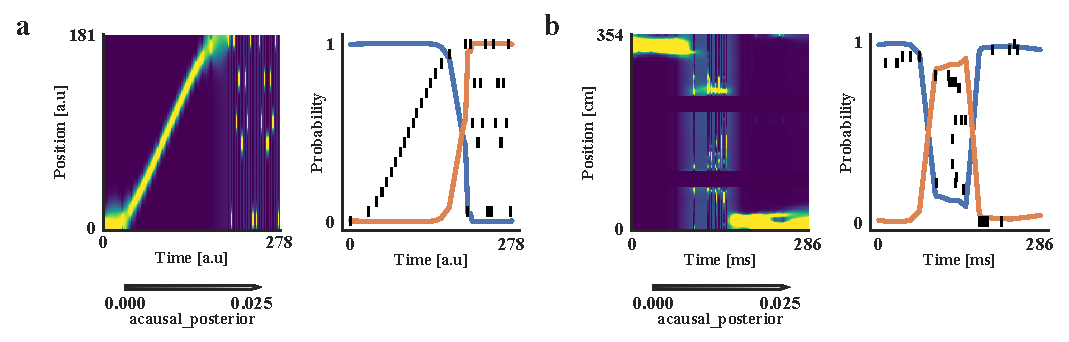
\includegraphics{fig1.pdf}}
\caption{The framework can be used to characterize changes between spatially continuous replay trajectories and spatially fragmented replay trajectories on simulated and real data. \textbf{(a)} The left plot shows a replay from 19 simulated neurons, arranged by the peak of their place fields, where the first three quarters of the replay is simulated to be spatially continuous and the last quarter is spatially fragmented. The black ticks indicate times when an action potential occurred. The blue and orange lines indicate the estimated probability of the continuous and fragmented discrete states over time $Pr(I_{k} \mid \Delta N_{1:T}^{(1:C)}, H_{k})$, respectively. The right plot shows the posterior probability of position represented by the neurons over time, marginalized over the discrete states $p(x_{k} \mid \Delta N_{1:T}^{(1:C)}, H_{k})$. \textbf{(b)} An example of how the model can capture similar patterns in real data from the spiking patterns of 32 hippocampal neurons during a sharp wave ripple. Conventions are the same as in the first plot. Positions in the right plot correspond to linearized position of a W-shaped track, where 0 cm corresponds to the top of the middle tine of the W, 354 cm corresponds to the top of the left tine of the W, and 212 cm corresponds to the right tine of the W. The top of the center arm and bottoms of the left and right arm are connected.}
\label{fig1}
\end{figure}

Next we define the discrete state transition $Pr(I_{k} \mid I_{k-1})$. From previous studies, we expect continuous trajectory replays will remain continuous and fragmented trajectories will remain fragmented for at least the duration of a sharp wave ripple. So, we define the probability of switching between fragmented and continuous or vice versa as low probability events and the probability of staying in either the fragmented or continuous state as high:
\begin{equation}
    Pr(I_{k} \mid I_{k-1}) = \begin{cases}
    0.999, \text{if } I_{k} = I_{k-1}; \\
    0.001, \text{if } I_{k} \ne I_{k-1};
    \end{cases}
\end{equation}{}

Lastly, we define the likelihood $p(\Delta N_{k}^{(1:C)} \mid x_{k}, I_{k}, H_{k})$ as the same in both conditions and the initial conditions to be uniform. This reflects that we do not have any prior knowledge about the starting position of the replay or differences in the place field representations.

To verify that this model works, we first simulate 19 inhomogeneous Poisson neurons with place fields spaced 10 arbitrary units (a.u.) along a 181 a.u linear track. These place fields have a standard deviation of 6 a.u. We then simulate a continuous trajectory replay---that is a replay that moves in a spatially continuous trajectory---and followed immediately by a fragmented replay--a replay that does not move in a spatially continuous trajectory (Fig.~\ref{fig1}a, left, black ticks). From Fig.~\ref{fig1}a, we can see that the model can track these changes in dynamics from the marginal probability of each discrete state. In the left plot, the probability of continuous trajectory (blue line) is high for the first three quarters of time in the simulated replay, because the spiking is highly sequential---indicating a continuous trajectory. As the spiking becomes non-sequential in the last quarter of time, the probability of the continuous state goes down and the probability of the fragmented state rises (orange line). This same pattern can be seen in the rightmost plot of Fig.~\ref{fig1}a, which displays the marginal position. The estimated position smoothly varies over time in the first three quarters of the replay and then changes to a discontinuous state in the latter quarter.

We can also find these same changes in dynamics from continuous trajectories to fragmented trajectories in real data. We use data previously published in \cite{KarlssonAwakereplayremote2009}. In Fig.~\ref{fig1}b, the model is fit to 32 neurons recorded from the hippocampus of a rat. The rat is performing a spatial alternation task in a W-shaped track. Place fields are fit with a Poisson generalized linear model using a b-spline basis over position to the spiking of the 32 neurons when the animal is running (times when the speed >4 cm/s). The random walk is modified to allow only allow transitions  to positions the animal has been on the track. All other transitions are set to zero. The left plot in Fig.~\ref{fig1}b shows the spiking during a sharp wave ripple event when the animal is stopped. The replay trajectory has a high probability of being continuous for the first third of the SWR, it then becomes more fragmented in the middle third of the SWR, and then transitions back to being continuous. From the right plot in Fig.~\ref{fig1}b, we can see that the position represented in this sharp wave ripple is at the top of the left of the W-track for the first third, many positions are represented for the middle third when the trajectory is fragmented, and then the top of the center arm is represented for the latter third of the SWR.

\subsection{Local vs. Non-Local Coding}
\begin{figure}[ht]
\centerline{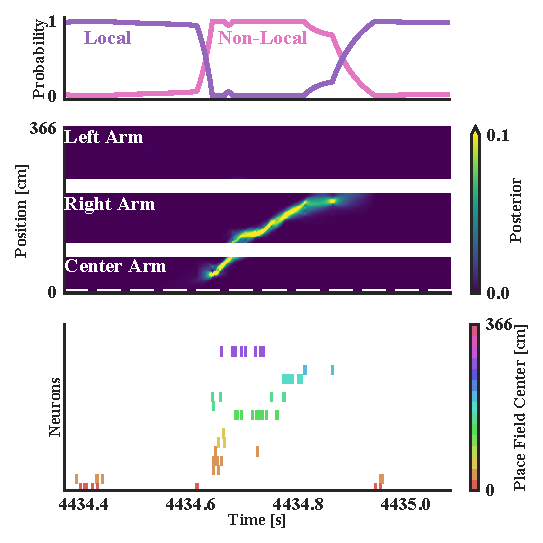
\includegraphics{fig2.pdf}}
\caption{An example of how the framework can be used to distinguish between local representations of position by the neurons---position that represents the animal's current location--and non-local trajectories on real data. The bottom plot shows spiking of 17 hippocampal neurons, arranged by linearized position and colored by the position that corresponds to the peak of their place field activity. The animal is at position 0. The top plot shows the estimated probability of the local and non-local discrete states over time $Pr(I_{k} \mid \Delta N_{1:T}^{(1:C)}, H_{k})$ in purple and pink respectively. The middle plot shows the posterior probability of position represented by the neurons over time, marginalized over the discrete states $p(x_{k} \mid \Delta N_{1:T}^{(1:C)}, H_{k})$. The white line in the middle plot indicates the animal's position. Position conventions are the same as in Fig.~\ref{fig1}b.}
\label{fig2}
\end{figure}

Now we show how the elements of the framework can be changed to answer a different question about replay. One of the defining features of replay is that it is an internally generated activity pattern that is different from the animal's behavior. This means that the neurons represent a position that is "non-local" to the animal's actual position in an environment. So it is of interest for neuroscientists to determine when the activity patterns of hippocampal neurons represent the animal's actual position versus a trajectory that does not represent the animal's position. Following \cite{EdenCharacterizingComplexMultiScale2018}, we can define two discrete states:
\begin{equation}
    I_{k} = \begin{cases}
        1, & \text{Local;}\\
        2, & \text{Non-local;}\\
         \end{cases}
\end{equation}

Notice that in this model, "local" means the position represented by the neurons corresponds to an observed variable---the position of the animal. If we define the animal's observed position at time $t_{k}$ as $m_{k}$, we can then define $\delta (m_{k})$ as an indicator function that denotes discretized position of the animal that changes with every time step. This can be used as a transition matrix that forces the transition to be the animal's actual position at each time step. Alternatively, we can think of this as just a discrete state with no continuous state transition associated that just uses the likelihood evaluated at the actual position of the animal at each time step. With the non-local state, we can again assume that corresponds to a continuous trajectory though the environment, so we can let the transitions within this state correspond to a random walk. With this, we can define the continuous state transition:
\begin{equation}
    p(x_{k} \mid x_{k-1}, I_{k}, I_{k-1}) = \begin{cases}
        \delta (m_{k}), & \text{if } I_{k}=1; \\
        \mathcal{U}(a, b), & \text{if } I_{k}=2, \\
        & \text{ and } I_{k-1}=1; \\
        \mathcal{N}(x_{k-1}, \sigma), & \text{if } I_{k}=2, \\
        & \text{ and } I_{k-1}=2;\\
        
    \end{cases}        
\end{equation}

For the discrete state transition, we can use our prior knowledge that sharp wave ripples are associated with non-local activity. Thus the probability of switching into the non-local state and staying in the non-local state will be approximately the same as the probability of switching into a sharp wave ripple and staying in the sharp wave ripple. We can fit a pair of logistic regression models to the detected sharp wave ripple as in \cite{EdenCharacterizingComplexMultiScale2018} to determine this switching probability empirically.
Finally, as in the previous example, we can set the likelihoods to be the same in each discrete state. For the initial conditions, we assume that we do not start in a non-local coding state. See \cite{EdenCharacterizingComplexMultiScale2018} for further details.

We can see again that this model can capture the features of interest when applied to real data. We fit the data on the same W-track experiment as the first example. In  Fig.~\ref{fig2}, the animal is at position 0---the top of the center arm---and we can see from the bottom plot that the spiking from 4434.4 seconds until 4434.6 seconds is from neurons that have place fields near position 0. The spiking from 4434.6 to 4434.8 seconds become non-local to the animal's position, representing a trajectory that moves down the center arm and up the right arm (Fig.~\ref{fig2}, middle plot). Just before 4435.0 seconds, the spiking activity pattern returns to representing the animal's position (Fig.~\ref{fig2}, bottom plot). We can see that the model nicely captures the timing of the local and non-local states by looking at the marginal probability of each state (Fig.~\ref{fig2}, bottom plot).

\section{Conclusion}
In this work, we have developed a point process state-space framework for understanding hippocampal replay that associates discrete latent states with continuous latent dynamics and allows for switching between the discrete states. We showed this framework is flexible: it can be deployed to characterize whether a replay represents spatially continuous trajectories or spatially discontinuous trajectories or it can be deployed to characterize local and non-local patterns of activity. Although we have only shown two examples of this framework, one could imagine combining the examples into one model---specifying that only during non-local states do we care about whether the trajectory is spatially continuous or not for example---or specifying more complicated conditions. All one has to specify is the initial condition, the likelihood, and state transition dynamic associated with each discrete state. The discrete state is then immediately interpretable in terms of the model. For example, the Poisson likelihood in the examples of this paper could easily be replaced by the marked point process likelihood in \cite{DengRapidclassificationhippocampal2016}---which would obviate the need for spike sorting before fitting the model.

This combination of interpretability and flexibility makes the framework is extremely powerful. By formulating what needs to be characterized mathematically, neuroscientists are forced to explicitly formulate their mental model of the replay characteristics of interest. This model can then be evaluated based on the data, criticized if the model assumptions are not adequate and improved into a better model. This iterative model building approach should be particularly powerful with respect to the hippocampus, where there are well-established features of the data and corresponding theories about the functioning of the hippocampus. The richness of data and theory about hippocampus could enable neuroscientists to take advantage of both the flexibility of the framework and the specificity that it allows.


\section*{Acknowledgments}
\printbibliography
\end{document}